

\chapter{Results}
In this chapter we show the results from our experiments on different types of imbalanced datasets. We first start by showing the results on the balanced model so as to set the baseline of comparisons. A discussion then follows on the under-sampled and over-sampled cases, ending with the transfer learning results for perturbations with different models. The chapter is then concluded with the results for the cases where classes have similar features, and, therefore, share overlapping distributions.


\section{Fully balanced model}

The objective of this research is to understand the effects of adversarial attacks on imbalanced CNNs. Canonical models assume that every object in the dataset are sampled from similar distributions. However, in real-life situations, even though the number of samples is the same, some class labels could be poorly represented by the lack of a clear structure. This could often lead to differences in the output for each specific class \cite{krawczyk2016learning}. On this way, a superficially balanced dataset does not guarantee that the model will equally generalise across all classes. Adversarial attacks were firstly done on a fully balanced model so as to use its results as baseline of comparisons for our imbalanced models.
\begin{figure}[H]
	\centering
	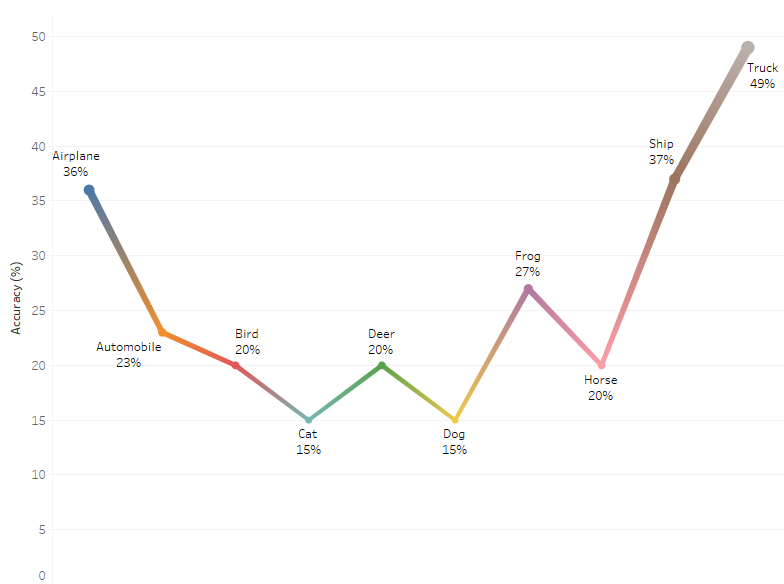
\includegraphics[scale=0.7]{balanced_perturbed.png}
	\caption{Individual class perturbed accuracy on the balanced model}
	\label{fig:balanced_perturbed}
\end{figure}

Figure ~\ref{fig:balanced_perturbed} shows that the accuracy for all classes is drastically reduced when the balanced model is presented with adversarial examples. Even though there is enough samples for each class, the adversarial attack forces the domain shift of each individual sample towards different regions in space, causing a misclassification of the current label. The effectiveness of the adversarial attack can be partially explained by the balancing of the dataset itself. In a model where the dataset used in training aims for normalization over all classes, the network is often caught in trying to find weights and biases that generalises well over all set of labels. Therefore, perturbations become more efficient due to a bigger proximity of classes distributions in space.


\section{Class under-sampling and over-sampling}


As the number of samples on a target class goes down, an increase of vulnerability towards that specific label is expected when compared to the balanced model. The results on table  ~\ref{tbl:results} confirms this. Networks with imbalanced datasets were more vulnerable when presented with adversarial examples. Figure ~\ref{fig:relative_difference} shows the relative difference for all the three networks (balanced, under-sampled and over-sampled).  The values were calculated by finding the difference between the new accuracy and the non-perturbed accuracy. They represent the percentage on which the initial accuracy was reduced. The under-sampled model had the higher relative difference on average, which shows that the imbalanced nature of the dataset ended-up increasing the vulnerability of the model. This poses threats to current systems as the low amount of samples during training for a specific class would  create gaps that are more easily exploited when compared to a balanced network. For instance, the decision boundaries of distributions are affected by the number of samples on the training set and, thus, can change model performance across each class.

Class imbalanced models are naturally affected by the false positive and false negative trade off shown on figure \ref{fig:class_dist}. The decision boundaries on such models favour the class with more samples and, hence, increases the accuracy for one class while decreasing for the other class. The area under the curve for misclassified examples on the under-sampled distribution is bigger, and it is caused by the suboptimal exploration of feature space of that class. This effect is exploited by adversaries as there is an increase on the misclassification rate of distributions with lower amplitude. An under-sample of a specific label causes its distribution to be squished into space and, hence, have less impact on the definition of decision boundaries.

\begin{figure}[H]
	\centering
	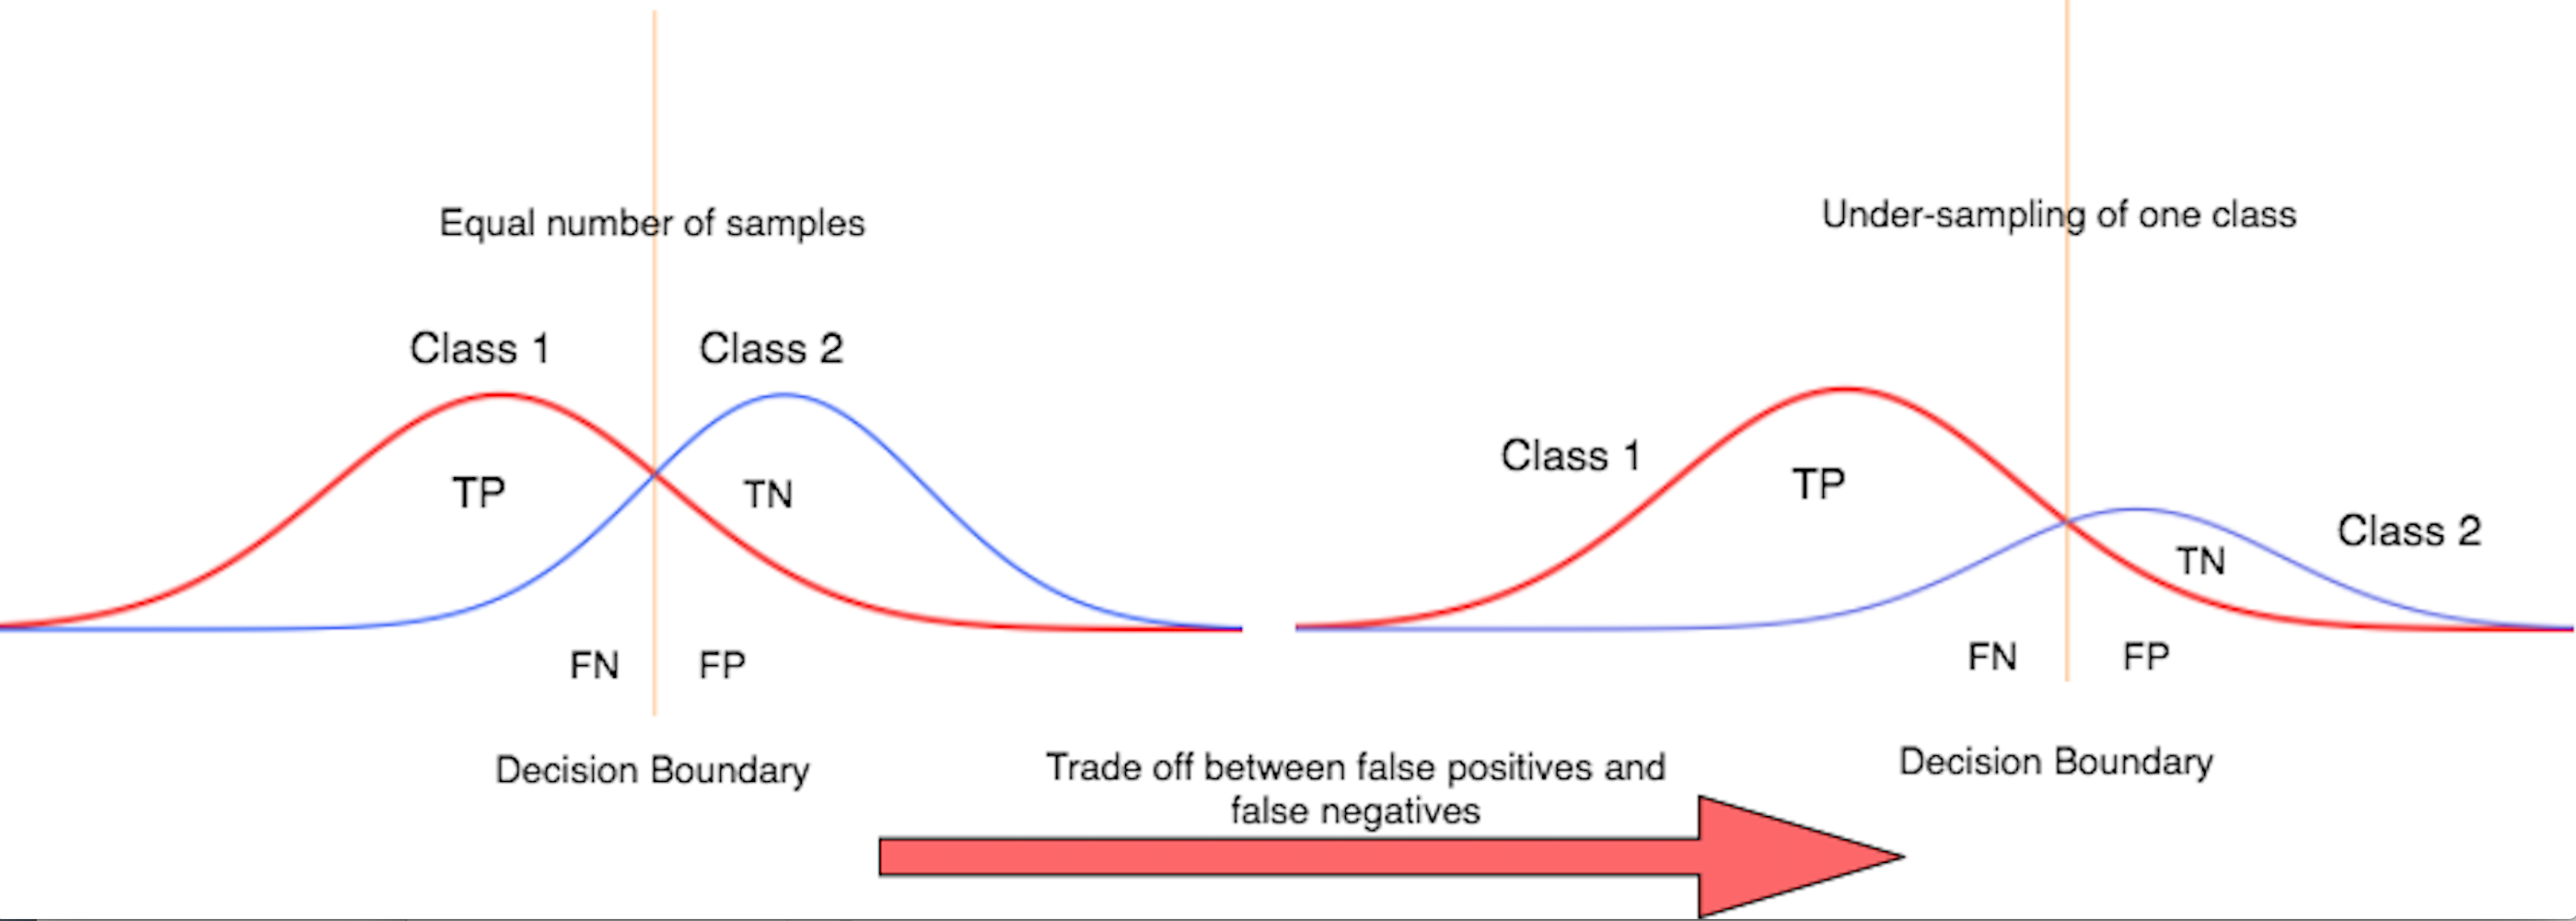
\includegraphics[scale=0.32]{class_dist.png}
	\caption{Dataset imbalance causes models to perform adjustments of decision boundaries leading to an increase on accuracy of the majority class and decrease on the minority class.}
	\label{fig:class_dist}
\end{figure}



\begin{table}[H]
	\centering
	
	\begin{tabular}{lccccc}
		\toprule
		&\multicolumn{2}{c}{Different Model}
		&\multicolumn{3}{c}{Same Model}
		\\\cmidrule(r){2-3}\cmidrule(l){4-6}
		Class Label &Undersample &Oversample &Balanced &Undersample &Oversample \\
		\midrule
		0 - Airplane &60\%& 87\% &36\%& 19\%    & 61\% \\
		1 - Automobile &64\%& 91\% &23\%& 16\%    & 63\% \\
		2 - Bird &38\%& 73\% &20\%& 9.4\%    & 27\% \\
		3 - Cat &21\%& 72\% &11\%& 0.5\%    & 19\% \\
		4 - Deer &58\%& 80\% &20\%& 9.8\%    & 20\% \\
		5 - Dog &47\%& 76\% &15\%& 9\%    & 38\% \\
		6 - Frog &76\%& 88\% &27\%& 20\%    & 49\% \\
		7 - Horse &59\%& 88\% &20\%& 18\%    & 52\% \\
		8 - Ship &69\%& 89\% &37\%& 19\%    & 59\% \\
		9 - Truck &46\%& 87\% &49\%& 21\%    & 54\% \\
		\bottomrule
	\end{tabular}
	\caption{Results for the two different sources of perturbations along with the two different imbalanced datasets}
	\label{tbl:results}
\end{table}

On the over-sampling case, the classes with more samples will naturally have higher overall influence when compared to classes with lower number of samples. This happens as the network performs more gradient updates on that specific class due to the amount of available samples. Perturbation on this case had a lower effect, as the small push caused by our $\epsilon$ was not enough to move points to outside of their distributions. Objects of the over-sampled classes would need bigger steps in order to successfully create an adversarial that leads to a misclassification output. Accuracy for most cases of the over-sampling case was around 45\% and the relative difference was the lowest of all three models, which shows robustness towards the target class. This approach can be used to increase system robustness on a specific label. For instance an application could have the desire to make a class stronger than the others due to critical factors on the classification of that label.

The increased number of samples of the over-sampled label, causes the network to perform a trade-off when optimizing its loss function. For instance, the decision boundary would be chosen in order to minimize the total error of the network. The cost function is lower when the decision boundary minimizes the misclassification of the majority class, as there is a higher number of samples. This phenomenon is well explained by figure ~\ref{fig:class_dist}, as the intersection of both distributions causes the densities to be different when we change the dataset balance.

\begin{figure}[H]
	\centering
	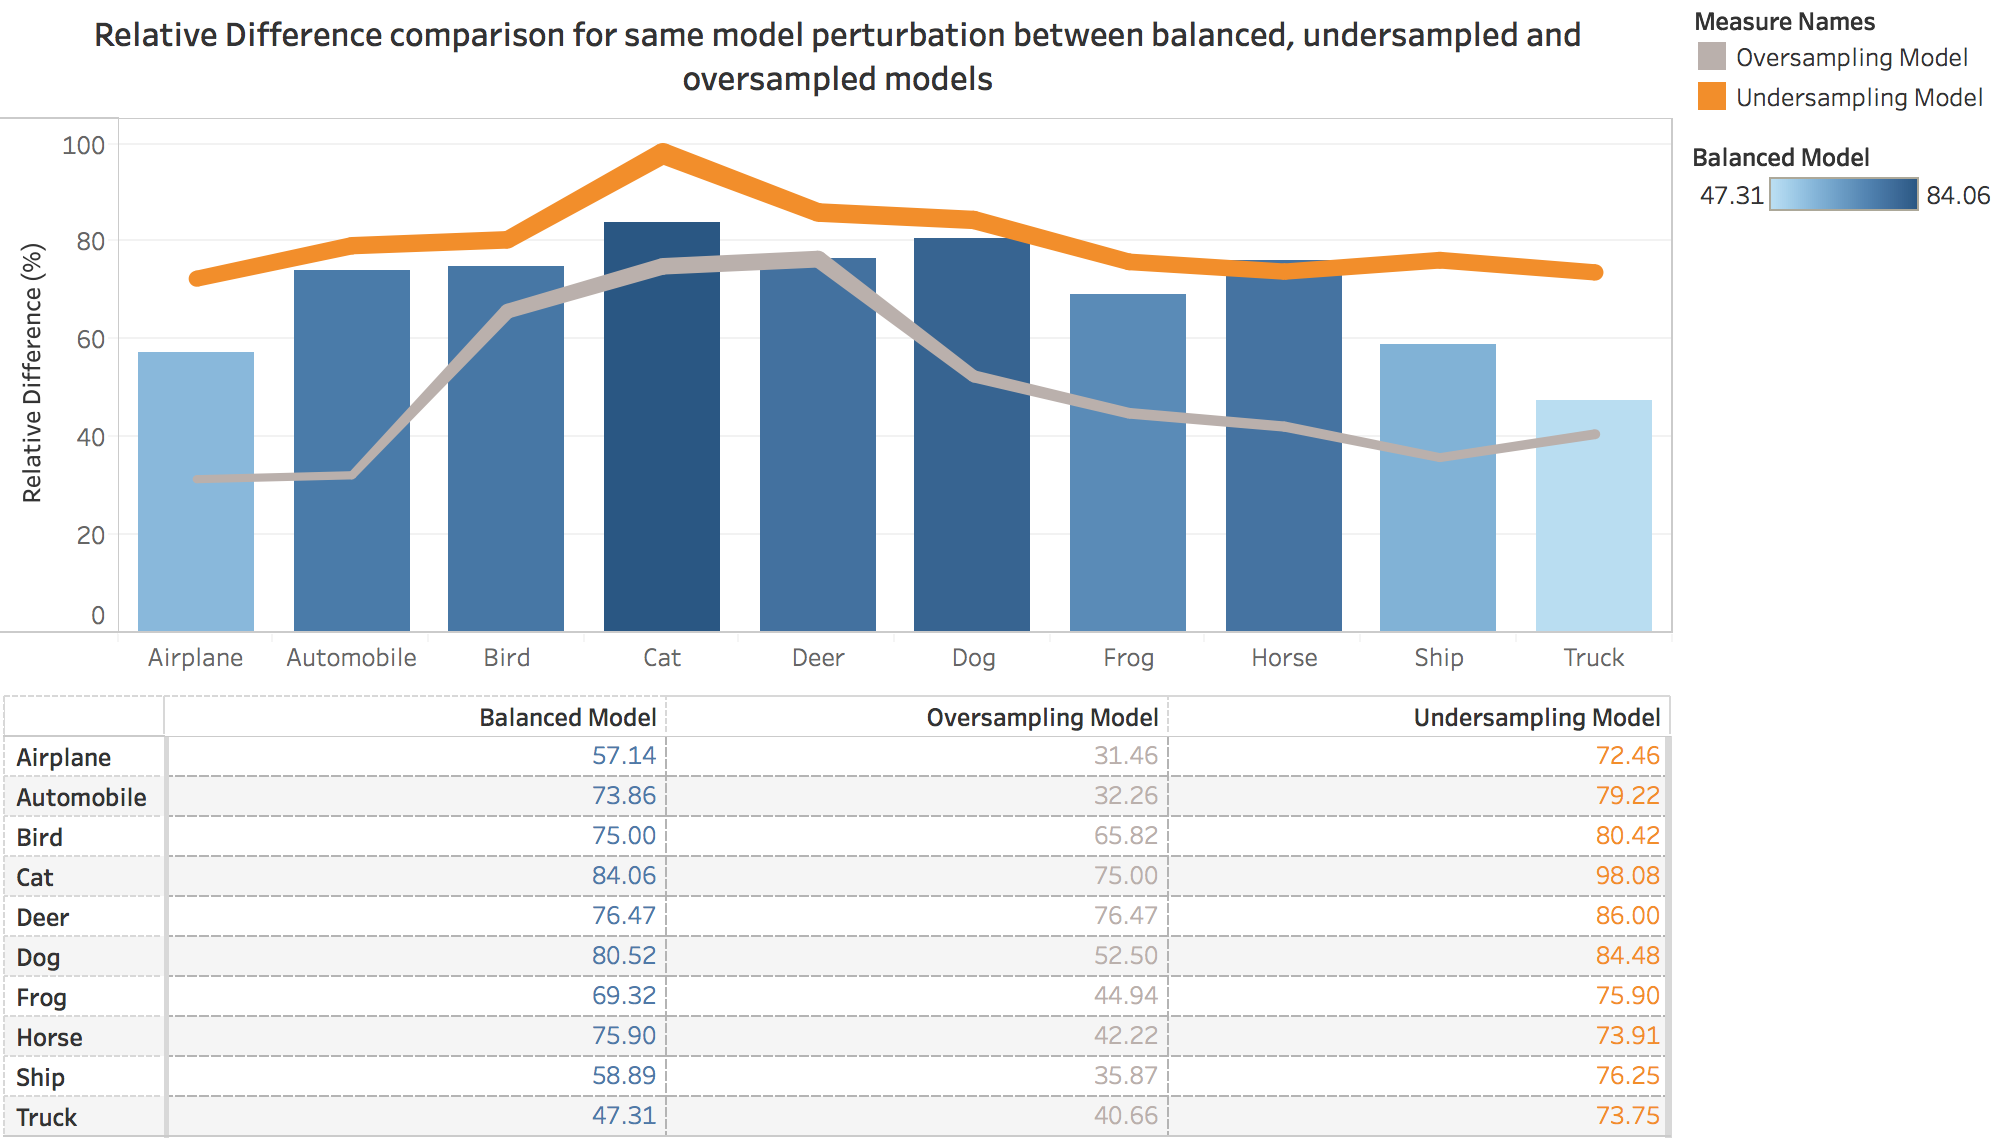
\includegraphics[scale=0.3]{rel_diff_graph.png}
	\caption{Relative difference for each model. Higher numbers means more vulnerability}
	\label{fig:relative_difference}
\end{figure}

\section{Transfer Learning}

Chapter 4 discussed different ways in which one algorithm could learn from existing models. When the attacker has no knowledge of the underlying model that he/she wants to attack, the best way to learn the gradient information is by querying the target and training a new model with its outputs. The use of a different model for creating adversaries has shown less effective when compared to the same model attack. As the overall gradient have not only different direction but also magnitudes, the attacked system has proven to be more robust. The experiment reveals that although Gradient Sign is quite effective for fooling networks it does require a good amount of knowledge from the underlying training parameters so as to unleash its full potential.

Attacking an under-sampled network with the gradient of the balanced network did not show to be as effective as using the same model's gradient. The average accuracy of an under-sampled model attack with adversaries generated from a different network was 53.8\% while the same metric was 25.8\% for the same model attack. Even that our training samples are within the same data domain, there are still huge differences on the gradients learned from the network. 

\section{Overlapping distributions}
When classes in the dataset already have distributions that are very close to one another the effects of adversaries seems to be even stronger. Figure ~\ref{fig:conf_matrix_full} shows that for the pairs cat and dog and automobile and truck, misclassification naturally happens towards one another due to similarities in their feature space \cite{stanford2016}. On this case, our experiment shows that the adversarial attacks intensifies this property by increasing the number on which one class is picked over another. Figure \ref{fig:overlap} shows that both cat and dogs are increasingly misclassified between themselves when imbalanced datasets on both classes are used. While on the cat under-sampling case 40\% of the samples were misclassified as dogs, on the oversampling 39\% of the dogs were misclassified as cats. This results gives interesting insights, as it shows that the gradient sign is navigating around the target class distribution and when an overlap occurs it becomes easier to create an adversarial to the class with higher similarities.

\begin{figure}[ht] 
	\label{fig7} 
	\begin{minipage}[b]{0.5\linewidth}
		\centering
		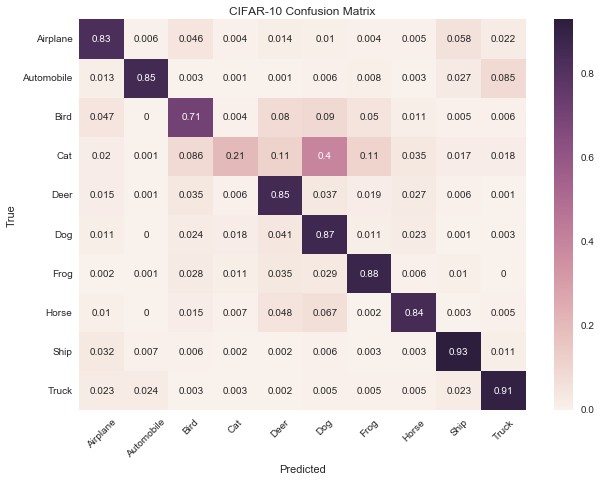
\includegraphics[width=1\linewidth]{cat_undersampling_per.png} 
		\vspace{4ex}
	\end{minipage}%%
	\begin{minipage}[b]{0.5\linewidth}
		\centering
		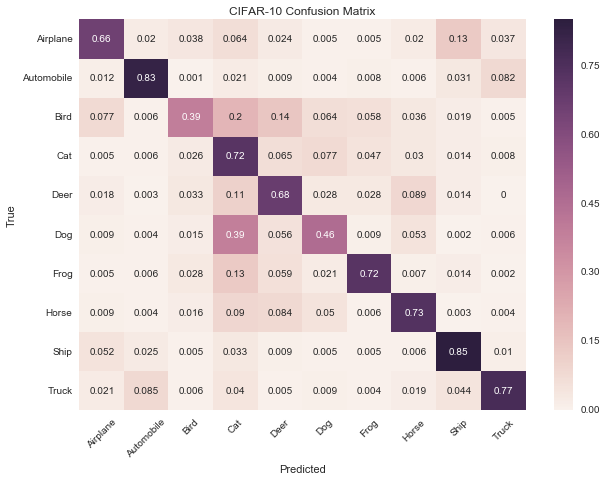
\includegraphics[width=1\linewidth]{cat_oversampling_per.png} 
		\vspace{4ex}
	\end{minipage} 
	\begin{minipage}[b]{0.5\linewidth}
		\centering
		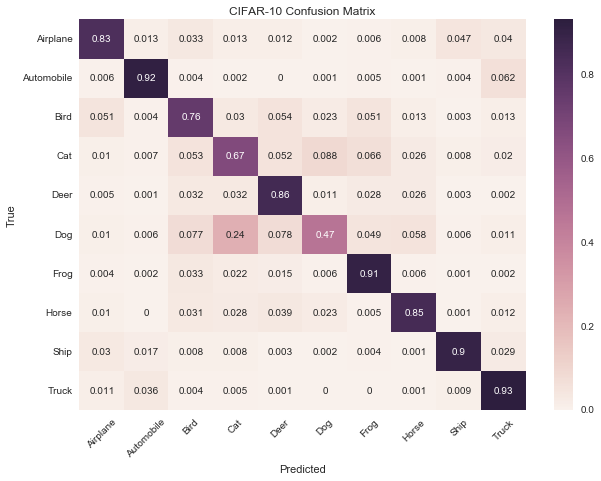
\includegraphics[width=1\linewidth]{dog_undersampling_per.png} 
		\vspace{4ex}
	\end{minipage}%% 
	\begin{minipage}[b]{0.5\linewidth}
		\centering
		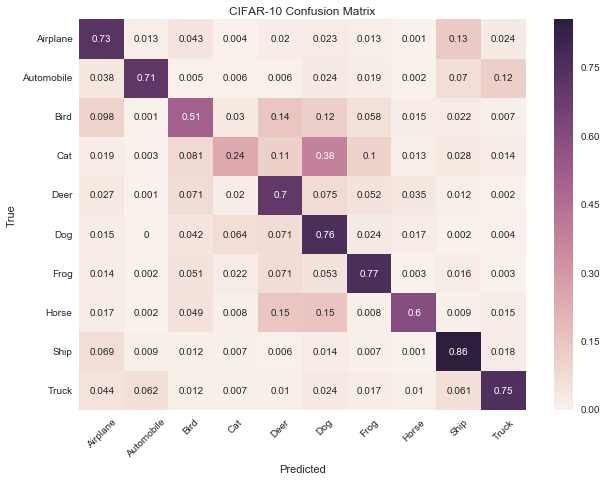
\includegraphics[width=1\linewidth]{dog_oversampling_per.png} 
		\vspace{4ex}
	\end{minipage} 
	\centering
	\caption{Top Left and Right: Cat undersampling / oversampling with perturbation. Bottom Left and Right: Dog undersampling / oversampling with perturbation}
	\label{fig:overlap}
\end{figure}

Classes with overlapping distributions sheds some light on the effect of the $\epsilon$ value of the gradient sign method. Its clear to understand that classes that are close together in the data space are required to take smaller steps in order to be successfully misclassified. Both dog and cat classes were already being confused with one another before the adversarial attack, and the small "push" of the gradient method has increased this effect, showing that domain shift is even stronger on these situations. The required amount of steps for classes with high level of uncertainty around them is often smaller when compared to classes with a better and more confident exploration of space.